% LFPformer -- NeurIPS 2026 poster
% Layout: Gemini beamerposter theme (https://github.com/anishathalye/gemini),
% NYU colour theme carried over from the Lfp2vec NeurIPS 2025 poster.
% Figures are cropped from the camera-ready paper (see figures/README.md).

\documentclass[final]{beamer}

% ====================
% Packages
% ====================
\usepackage[size=custom, width=120, height=80, scale=1.1]{beamerposter}
\usetheme{gemini}
\usecolortheme{cam}
\usepackage{graphicx}
\usepackage{booktabs}
\usepackage{amsmath}
\usepackage{tikz}
\usepackage{anyfontsize}
\usepackage{qrcode}

\setbeamerfont{itemize/enumerate body}{parent=normal text}
\setbeamerfont{itemize/enumerate subbody}{parent=normal text}
\setbeamerfont{block title}{family=\Raleway, series=\geminititleseries, size=\LARGE}
\setbeamerfont{block body}{family=\sffamily, size=\normalsize}
\setbeamerfont{normal text}{family=\sffamily, size=\normalsize}
\renewcommand{\familydefault}{\sfdefault}

% Paper colours for the pretraining objectives
\definecolor{maskpred}{HTML}{6E6E6E}
\definecolor{chandistc}{HTML}{0F8B8D}
\definecolor{manipdistc}{HTML}{882255}
\definecolor{ccfdistc}{HTML}{D4880F}
\newcommand{\MP}{\textcolor{maskpred}{\textbf{MaskPred}}}
\newcommand{\CD}{\textcolor{chandistc}{\textbf{ChanDistc}}}
\newcommand{\MD}{\textcolor{manipdistc}{\textbf{ManipDistc}}}
\newcommand{\CCF}{\textcolor{ccfdistc}{\textbf{CCFDistc}}}
\newcommand{\LF}{\textbf{LFPformer}}

% Highlighted take-away line under each figure
\newcommand{\takeaway}[1]{%
  \vspace{0.4ex}%
  \begin{beamercolorbox}[wd=\linewidth,sep=0.8ex,rounded=false]{takeaway}%
    \normalsize #1%
  \end{beamercolorbox}}
\setbeamercolor{takeaway}{fg=black,bg=nyupurple!8}

% ====================
% Lengths: 4 columns
% (N+1)*sepwidth + N*colwidth = paperwidth
% ====================
\newlength{\sepwidth}
\newlength{\colwidth}
\setlength{\sepwidth}{0.012\paperwidth}
\setlength{\colwidth}{0.235\paperwidth}
\newcommand{\separatorcolumn}{\begin{column}{\sepwidth}\end{column}}

% ====================
% Title
% ====================
\title{{\fontsize{64pt}{76pt}\selectfont LFPformer: Geometry-Aware Self-Supervised Electrophysiology Representation Learning}}

\author{{\fontsize{27pt}{32pt}\selectfont
  Subhrajit Dey\textsuperscript{1*},
  Ping-Jung Lu\textsuperscript{1*},
  Visweswar Sirish Parupudi\textsuperscript{1*},
  Malhar Patel\textsuperscript{1*},
  Margaret-Estefani Conde Paredes\textsuperscript{2},
  Mihály Vöröslakos\textsuperscript{3},
  Anna Maslarova\textsuperscript{3},
  György Buzsáki\textsuperscript{3},
  Saurabh Vyas\textsuperscript{4},
  Erdem Varol\textsuperscript{1,3}}}

\institute{{\fontsize{23pt}{28pt}\selectfont
  \textsuperscript{1}Department of Computer Science, New York University \quad
  \textsuperscript{2}Zuckerman Mind Brain Behavior Institute, Columbia University \\
  \textsuperscript{3}Neuroscience Institute, NYU Grossman School of Medicine \quad
  \textsuperscript{4}Neuroscience Institute \& Biomedical Engineering, Carnegie Mellon University
  \quad \textsuperscript{*}Equal contribution}}

% ====================
% Footer
% ====================
\footercontent{
  \makebox[0pt][l]{\href{https://github.com/neuroinfolab/LFPformer}{github.com/neuroinfolab/LFPformer}}
  \hfill
  \makebox[0pt]{\textbf{NeurIPS 2026}}
  \hfill
  \makebox[0pt][r]{\href{https://www.neuroinformaticslab.com/lfpformer}{neuroinformaticslab.com/lfpformer}}
}

% ====================
% Logos
% ====================
\logoleft{
\includegraphics[height=5.5cm]{logos/NYU_neuroinfo_logo.png}}
\logoright{
\includegraphics[height=5.5cm]{logos/NYU_langone.png}}

% ====================
% Body
% ====================
\begin{document}
\begin{frame}[t]
\begin{columns}[t]
\separatorcolumn

% ------------------------------------------------------------------ column 1
\begin{column}{\colwidth}

\begin{block}{Overview}
  \textbf{Question.} Can the \emph{acquisition geometry} of a recording (probe layout, insertion log) teach a foundation model where an LFP channel sits in the brain, with no histology during pretraining?

  \textbf{Approach.} \LF{} adds one geometry-aware contrastive loss to audio-pretrained wav2vec~2.0: chunks recorded close together are pulled together, distant ones pushed apart.

  \textbf{Findings.} Embeddings organise by anatomy, beat supervised spectrogram models at 3D localization, transfer across labs, probes and species, and track regional LFP spectra.
\end{block}

\begin{block}{Method}
  \centering
  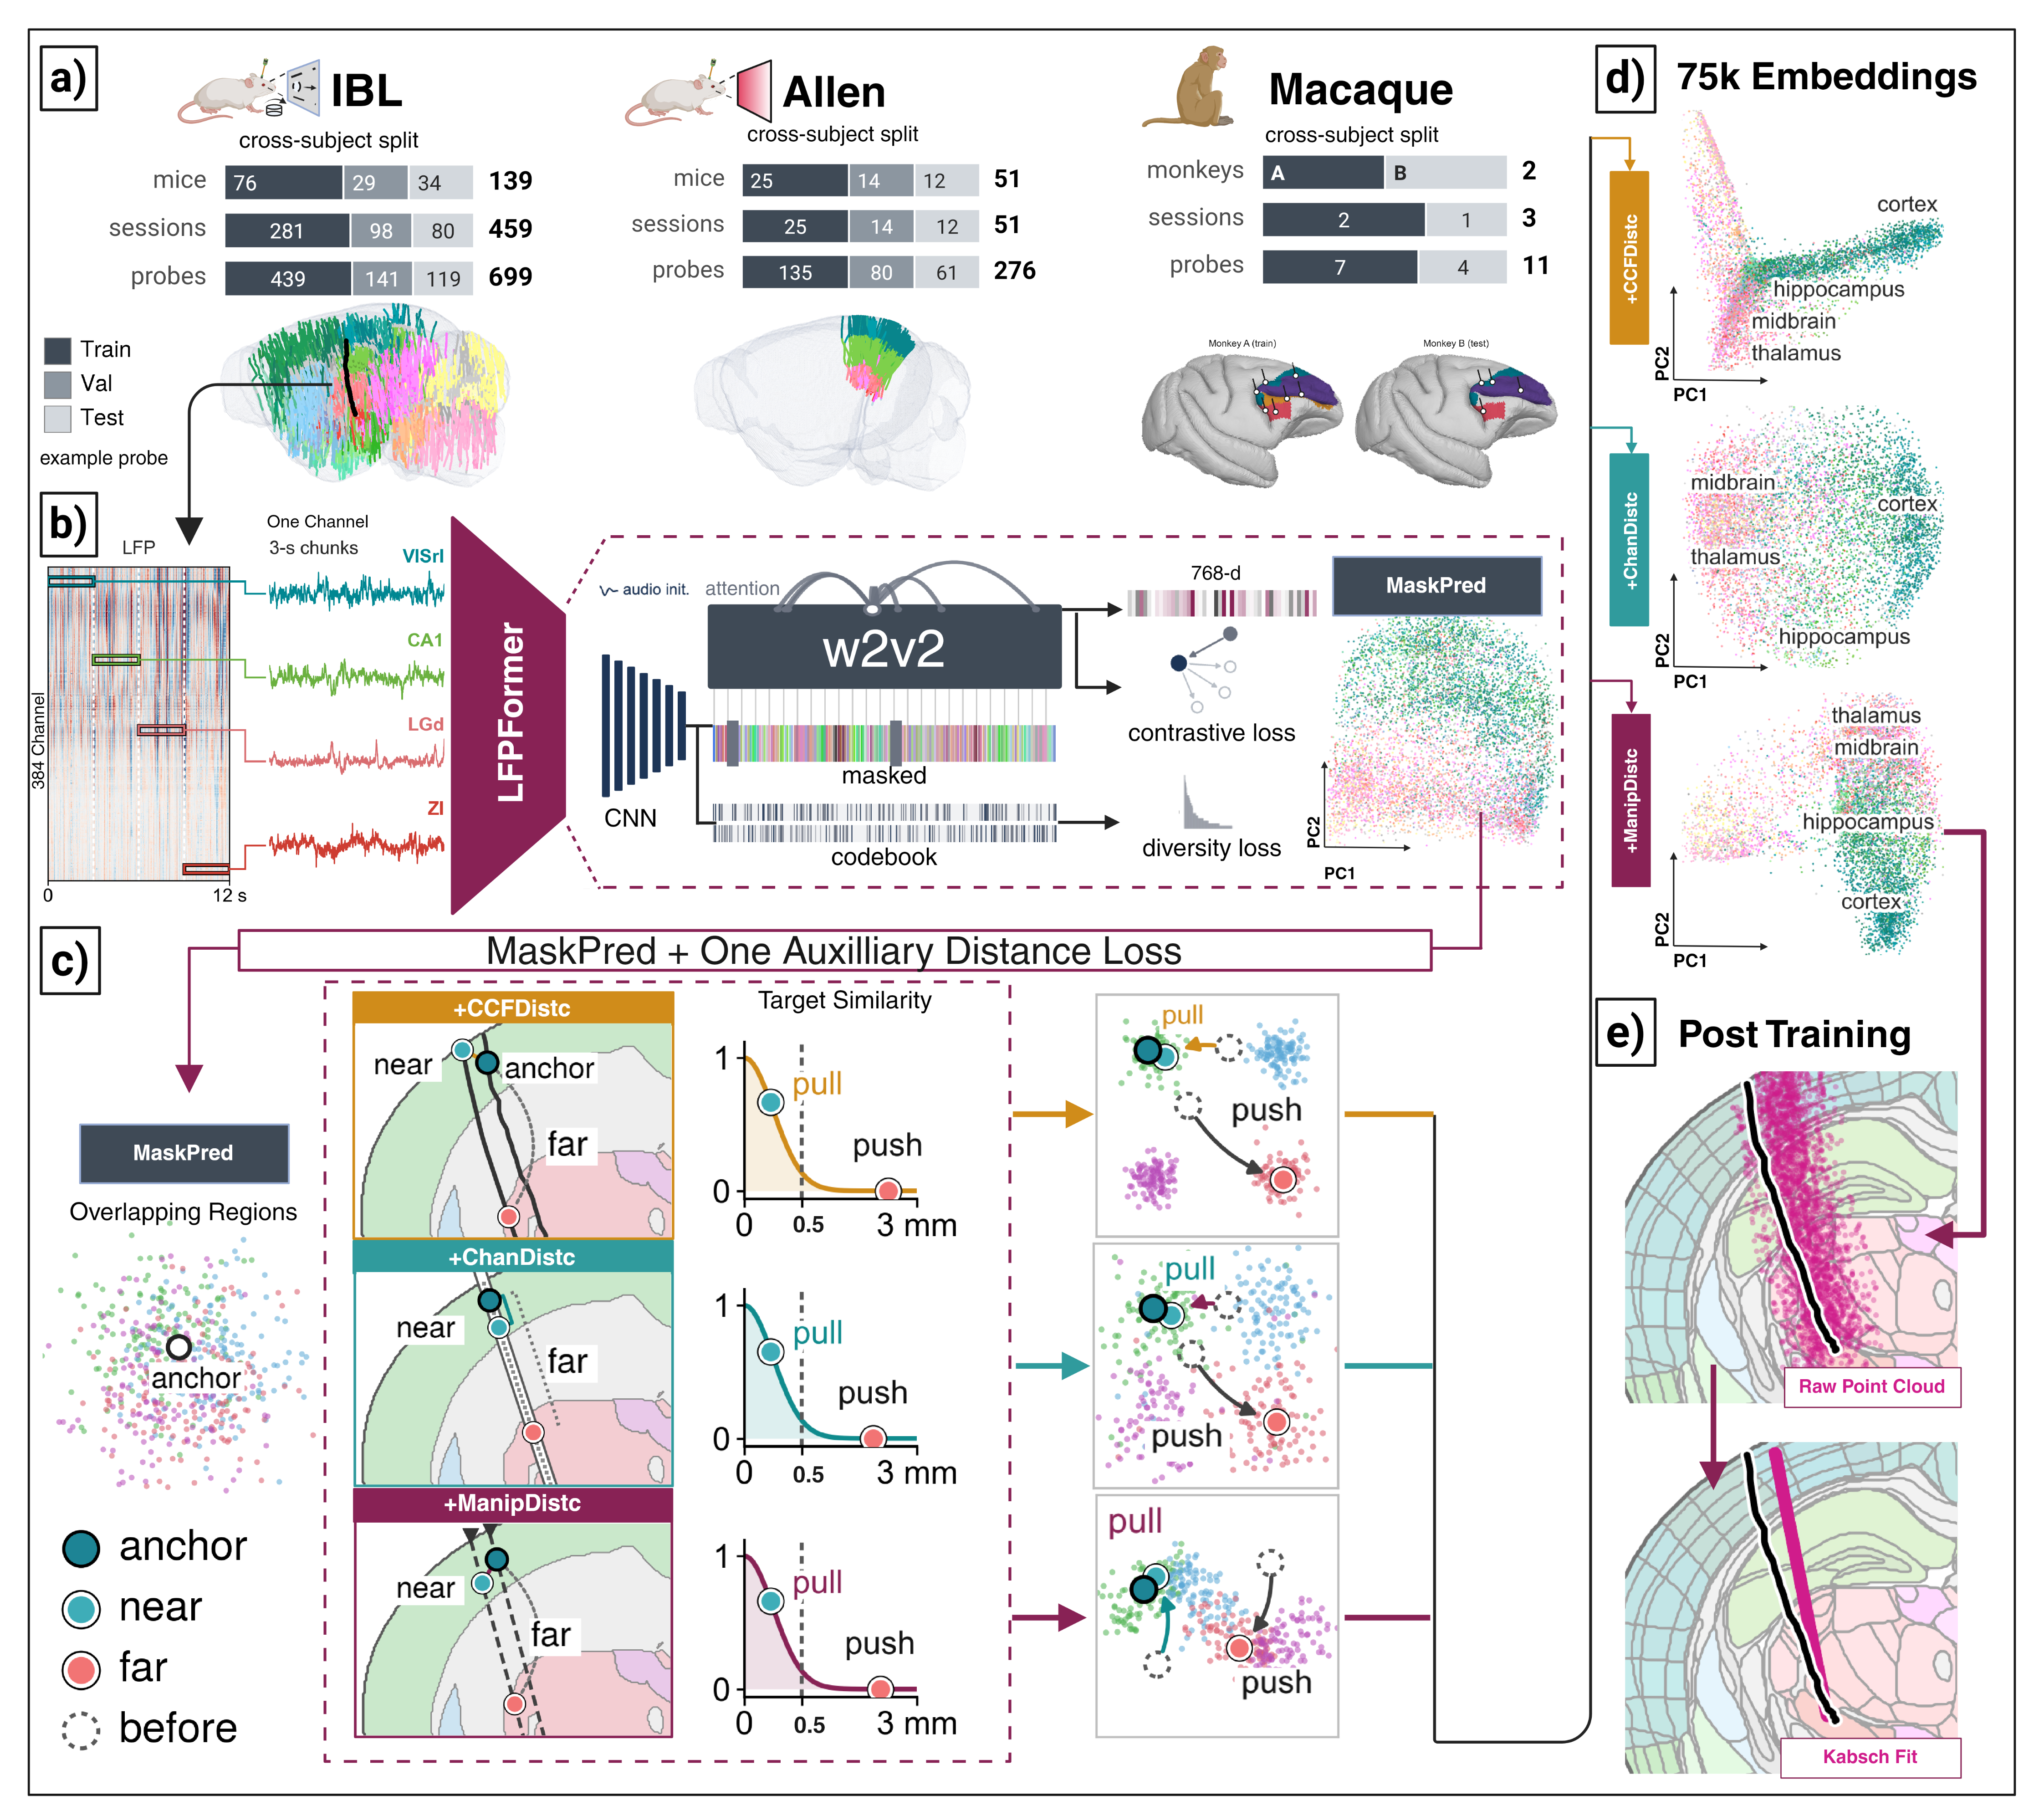
\includegraphics[width=\linewidth]{figures/fig1_overview.png}
  \raggedright

  \vspace{0.5ex}
  \textbf{Pretrain} on single-channel 3-s LFP chunks (IBL, Allen). Keep the wav2vec~2.0 objective (\MP) and add one spatial loss with target similarity $\exp(-d_{ij}^2/2\sigma^2)$, $\sigma=0.5$~mm:
  \[
    \mathcal{L}_{\text{pretrain}}
    = \underbrace{\mathcal{L}_{\text{contrast}} + 0.1\,\mathcal{L}_{\text{div}}}_{\text{MaskPred}}
    + \lambda_t\,\mathcal{L}_{\text{spatial}}
  \]
  The variants differ only in where $d_{ij}$ comes from:
  \begin{itemize}
    \item \CD: channel spacing on the probe itself
    \item \MD: insertion line from the micromanipulator log
    \item \CCF: histology coordinates (oracle reference)
  \end{itemize}

  \textbf{Read out} a mean and uncertainty per chunk (Gaussian NLL), \textbf{pool} per channel with weights $1/\hat\sigma^2$, and rigidly fit the known probe geometry (\textbf{Kabsch}); no test anatomy enters the fit.
\end{block}

\end{column}
\separatorcolumn

% ------------------------------------------------------------------ column 2
\begin{column}{\colwidth}

\begin{block}{3D Localization in Held-Out Mice}
  \centering
  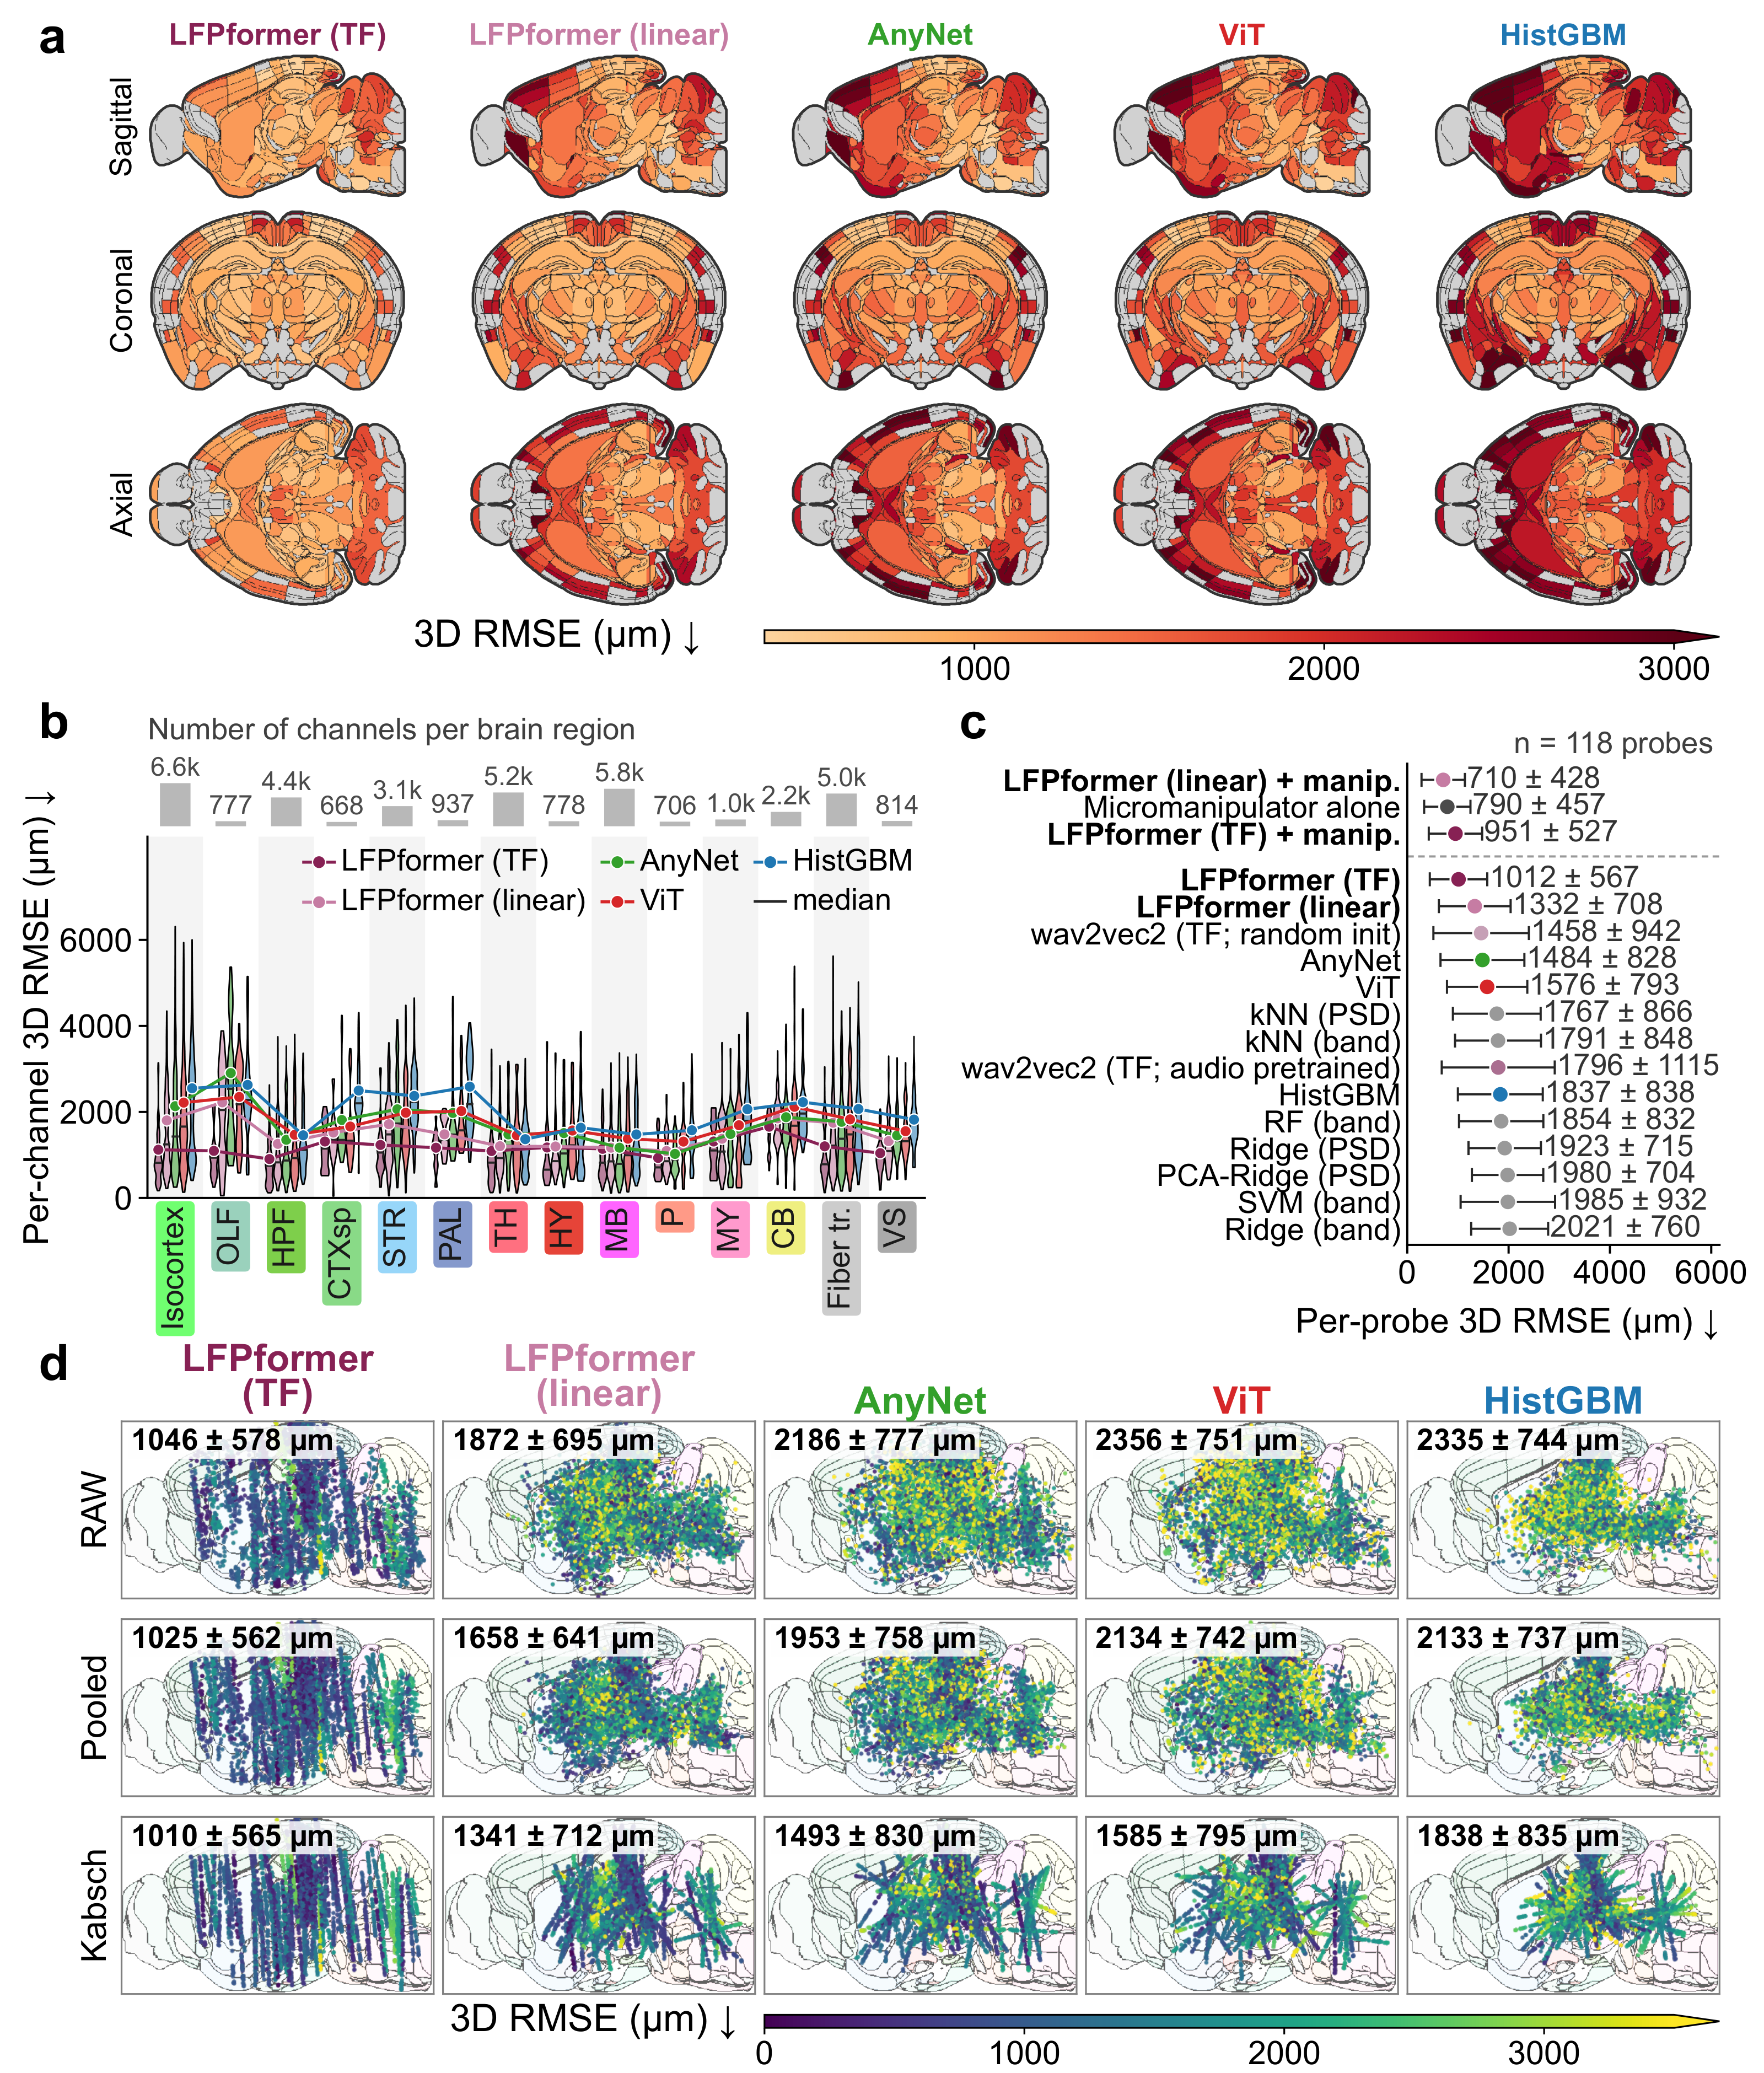
\includegraphics[width=0.92\linewidth]{figures/fig2ad_ibl_localization.png}
  \raggedright
  \vspace{-1.5ex}
  \begin{itemize}
    \item Frozen MaskPred+\MD{} encoder; per-probe 3D error over 118 probes: Transformer readout \textbf{1012~µm} vs.\ linear 1332, AnyNet 1484, ViT 1576~µm.
    \item Adding micromanipulator coordinates: \textbf{710~µm} vs.\ 790~µm for the micromanipulator alone.
  \end{itemize}
\end{block}

\begin{block}{Scaling Data, Decoders and Compute}
  \centering
  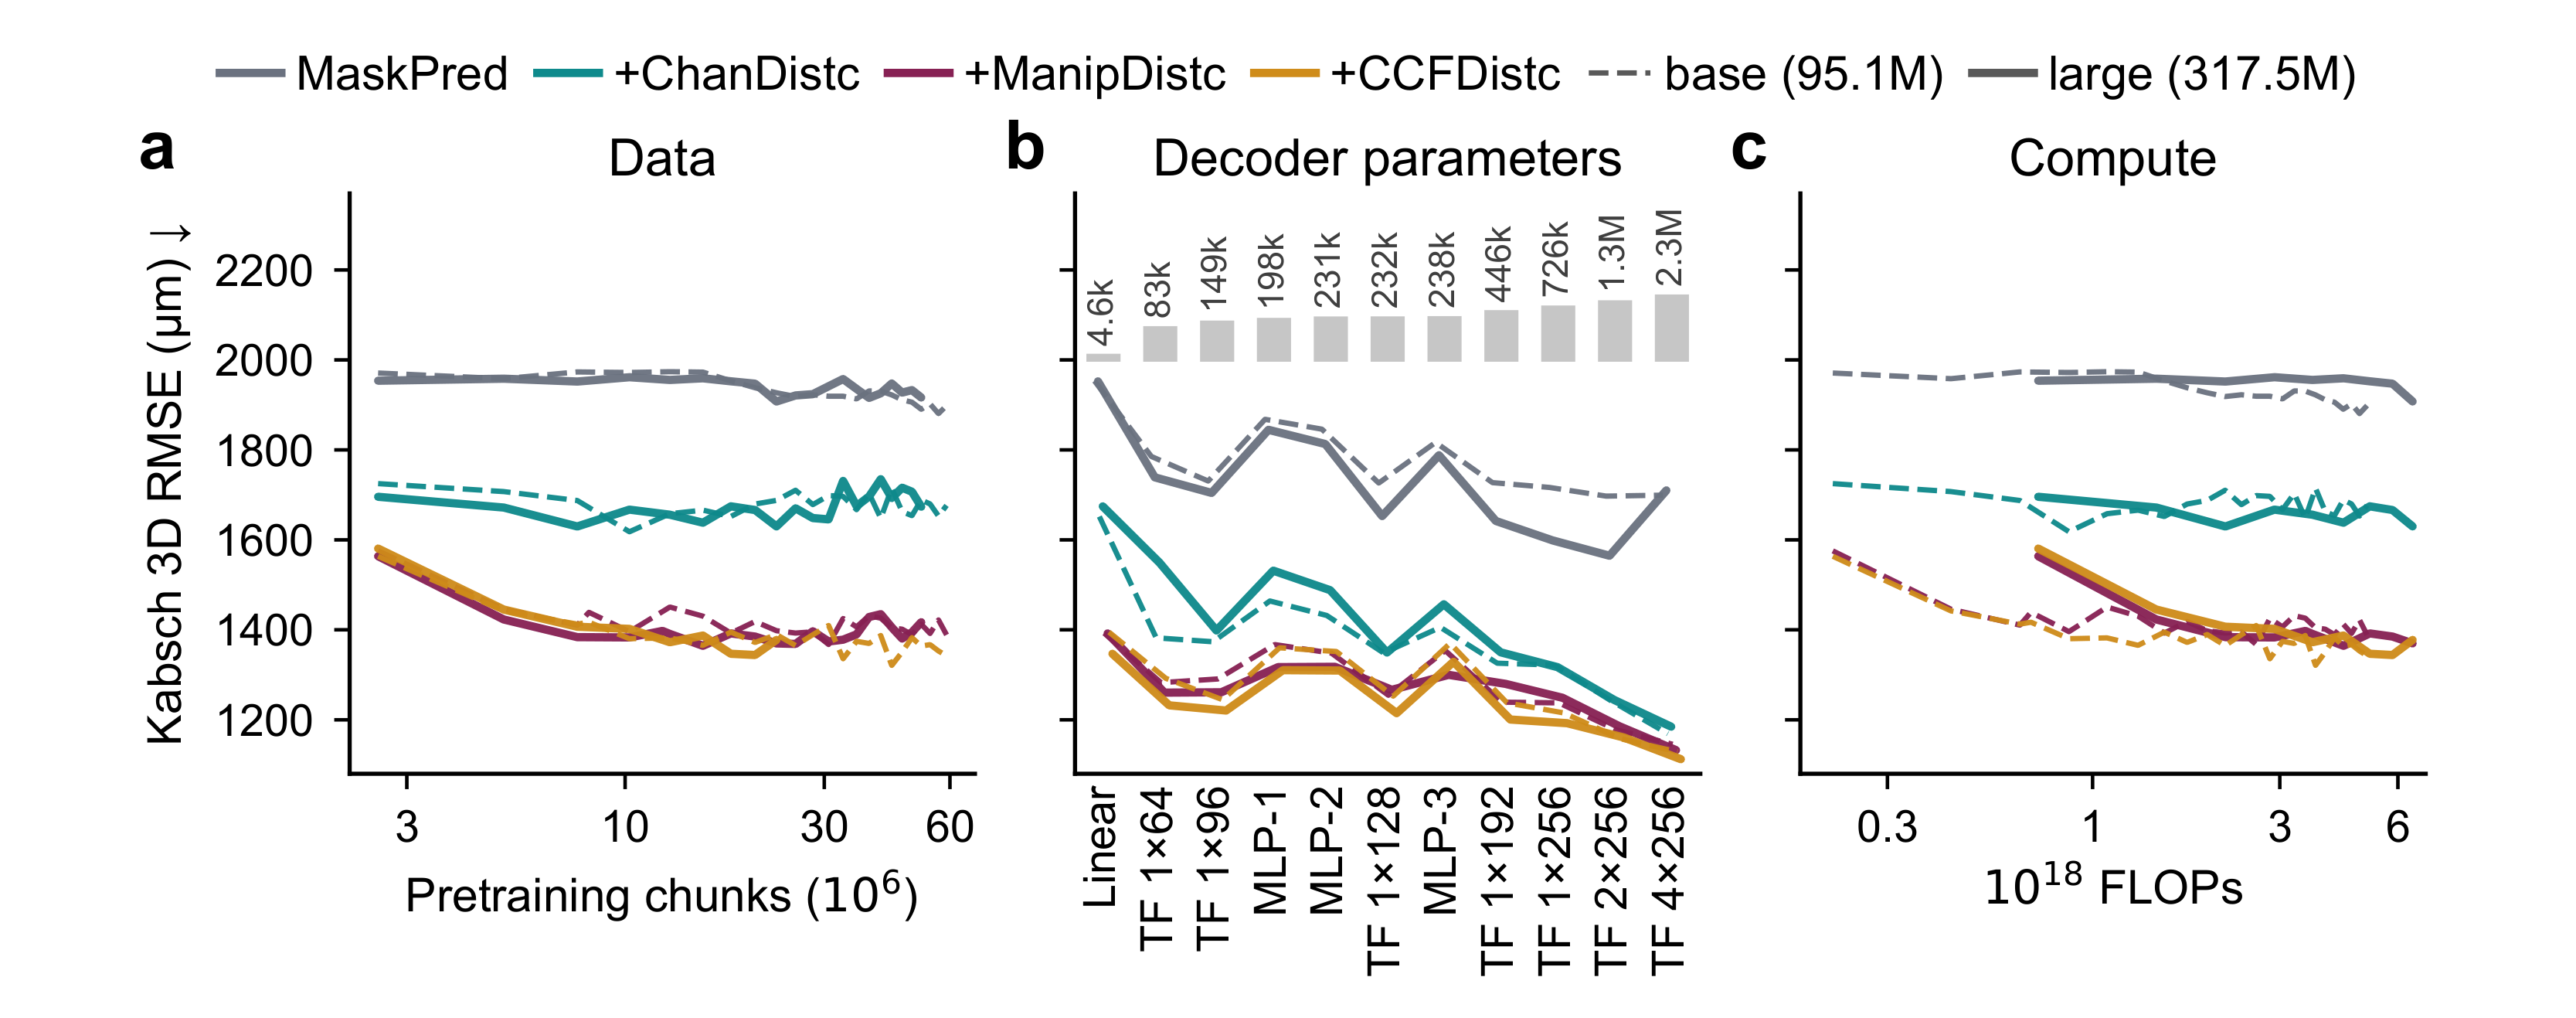
\includegraphics[width=\linewidth]{figures/fig4_scaling.png}
  \raggedright
  \vspace{-1.5ex}
  \begin{itemize}
    \item Up to 58.88M chunks; base (95.1M) vs.\ large (317.5M) encoders. \MD{} and \CCF{} improve early then plateau; Transformer readouts narrow the gap, and larger encoders do not consistently help.
  \end{itemize}
\end{block}

\end{column}
\separatorcolumn

% ------------------------------------------------------------------ column 3
\begin{column}{\colwidth}

\begin{block}{Brain Region Classification}
  \centering
  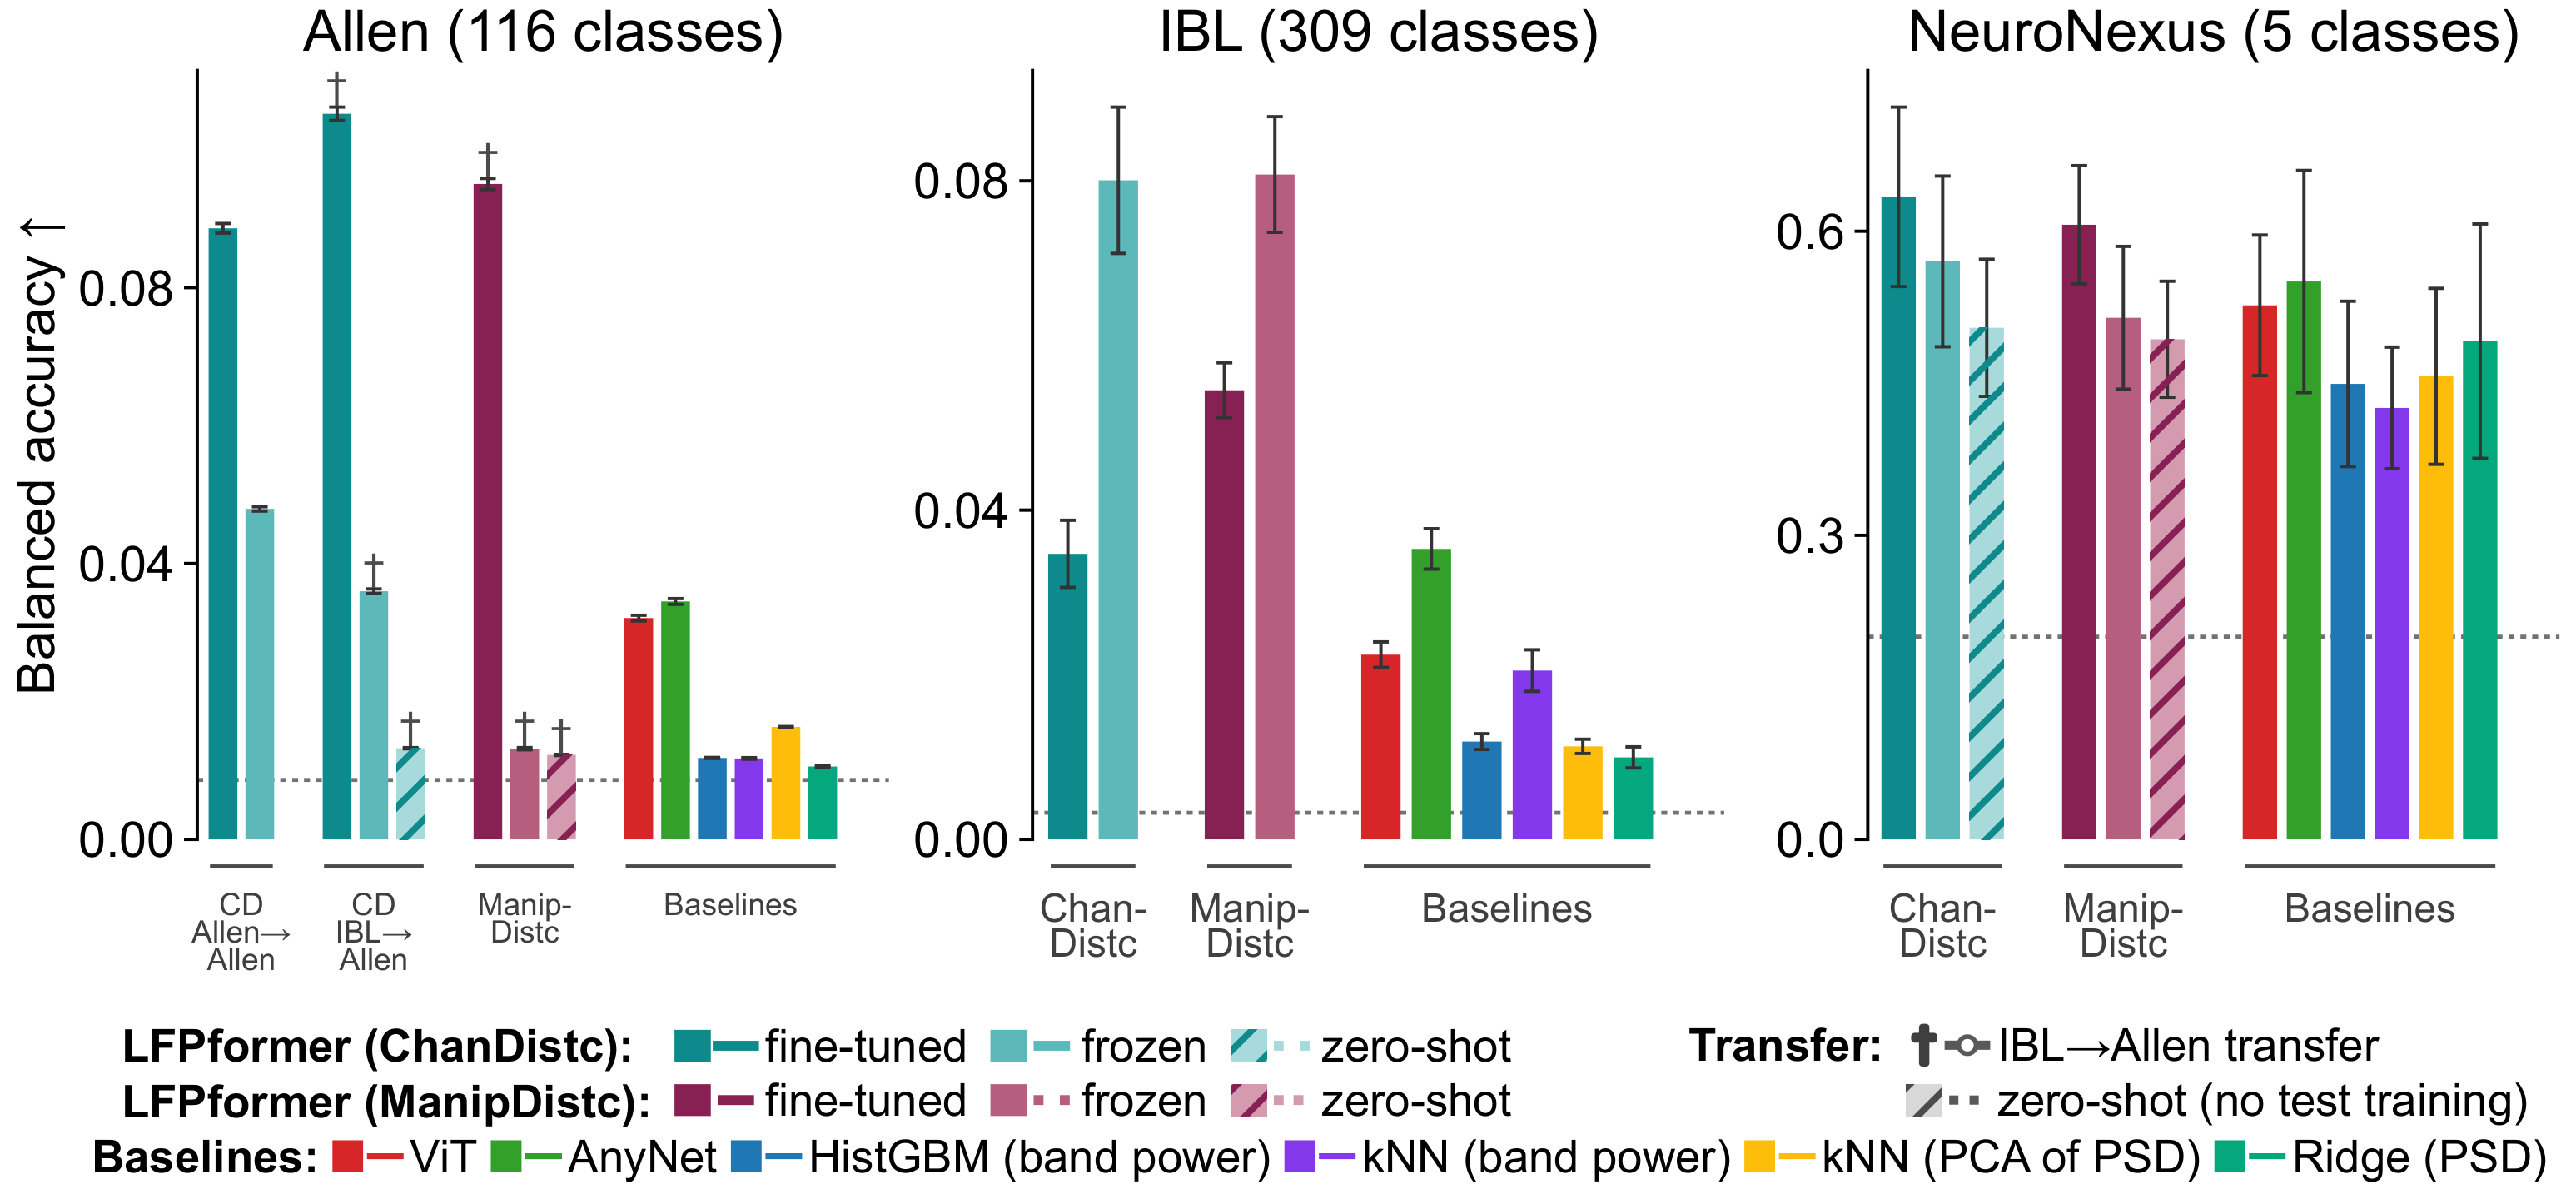
\includegraphics[width=\linewidth]{figures/fig3a_region_classification.png}
  \raggedright
  \vspace{-1.5ex}
  \begin{itemize}
    \item New probe type (NeuroNexus, 7 held-out sessions): fine-tuned \CD{} \textbf{0.634~$\pm$~0.089} balanced acc.\ vs.\ \MD{} 0.606, AnyNet 0.550, ViT 0.527.
    \item IBL-pretrained \CD{} beats Allen-pretrained \CD{} on Allen ($\dagger$).
  \end{itemize}
\end{block}

\begin{block}{Mouse-to-Macaque Transfer}
  \centering
  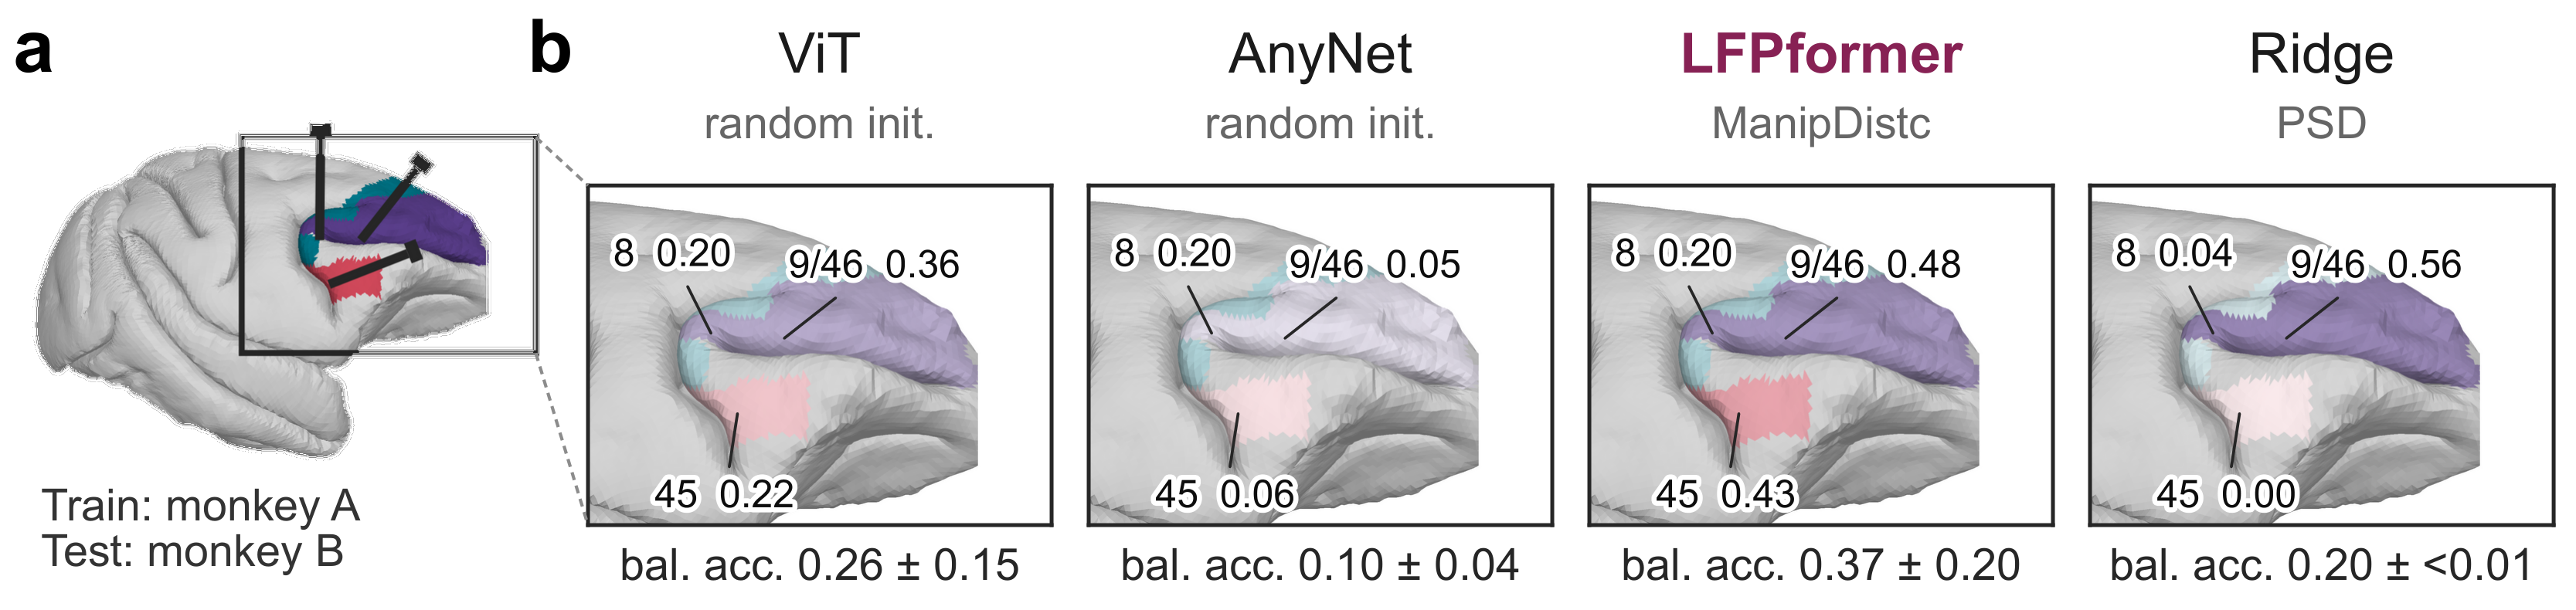
\includegraphics[width=\linewidth]{figures/supp_fig8ab_macaque.png}
  \raggedright
  \vspace{-1.5ex}
  \begin{itemize}
    \item Fine-tuned on monkey A, tested on monkey B: \MD{} \textbf{0.37~$\pm$~0.20} bal.\ acc.\ vs.\ ViT 0.26, Ridge 0.20 (2 animals).
  \end{itemize}
\end{block}

\begin{block}{Embeddings Follow LFP Spectra}
  \centering
  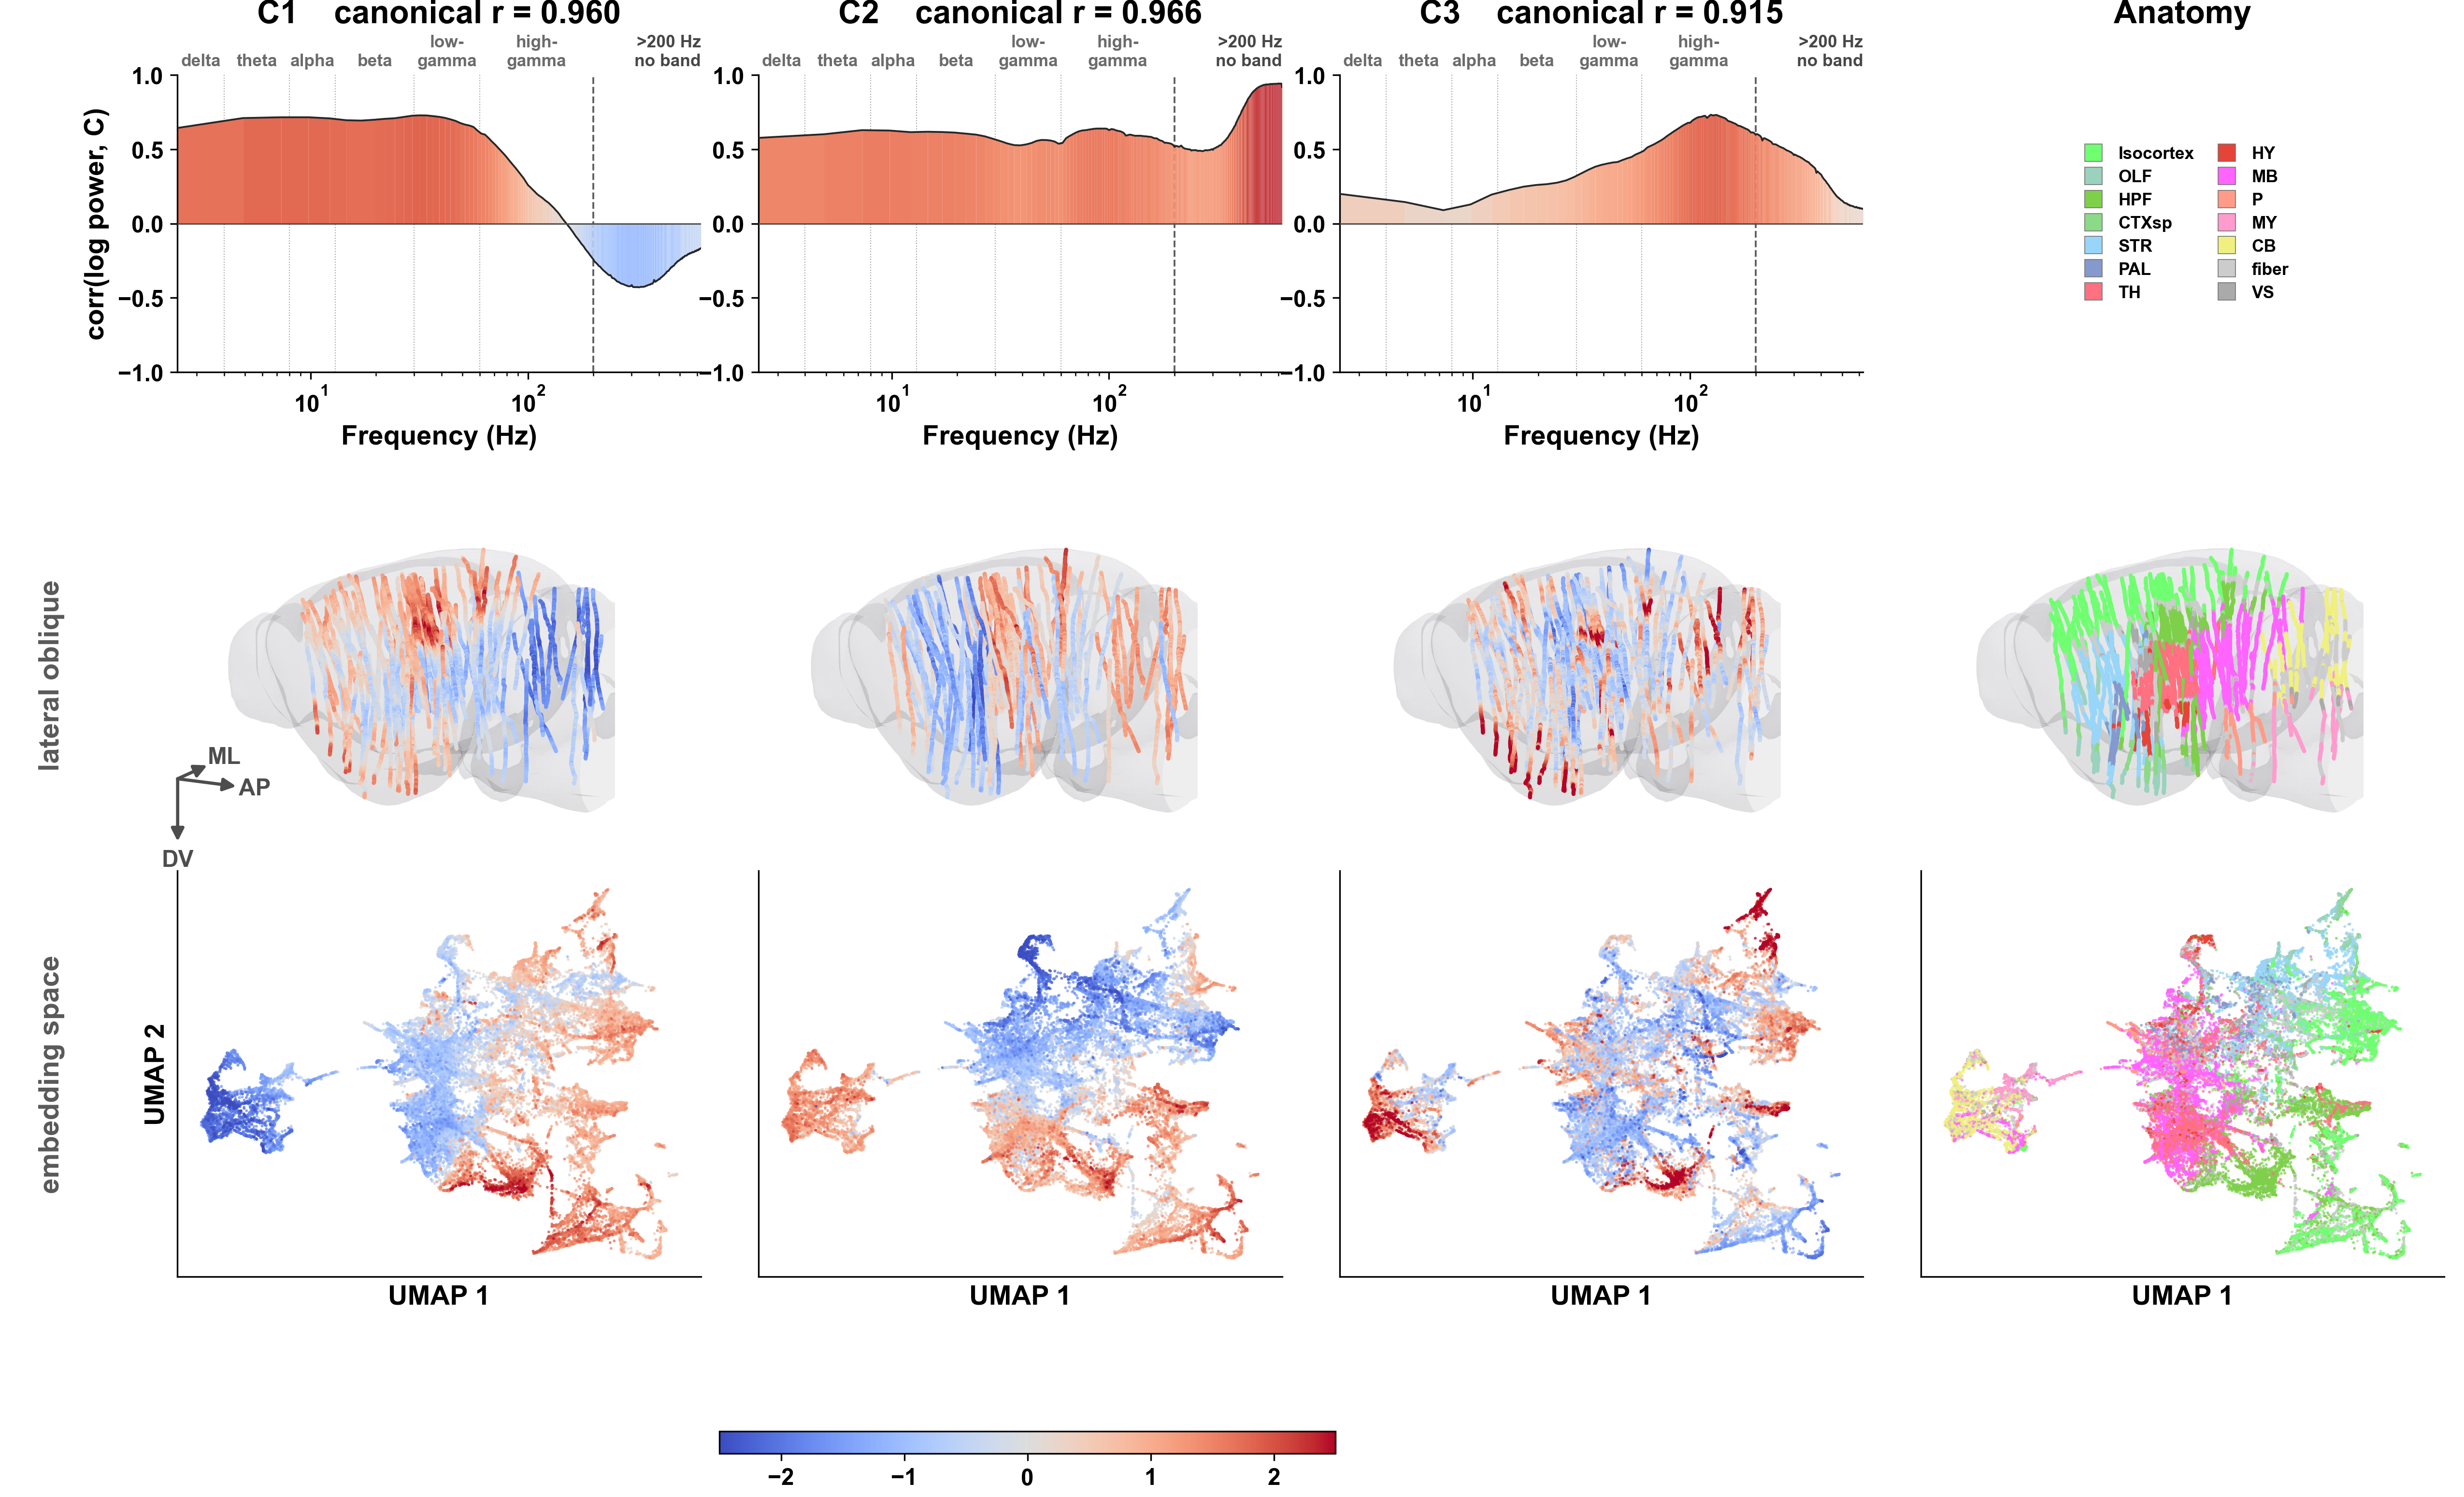
\includegraphics[width=0.9\linewidth]{figures/fig6_cca_spectra.png}
  \raggedright
  \vspace{-1.5ex}
  \begin{itemize}
    \item CCA of frozen embeddings vs.\ per-channel log power spectra (39,615 channels). C1: low frequency vs.\ $>$200~Hz; C2: broadband; C3: high gamma.
  \end{itemize}
\end{block}

\end{column}
\separatorcolumn

% ------------------------------------------------------------------ column 4
\begin{column}{\colwidth}

\begin{block}{Zero-Shot on a Chronic Implant}
  \centering
  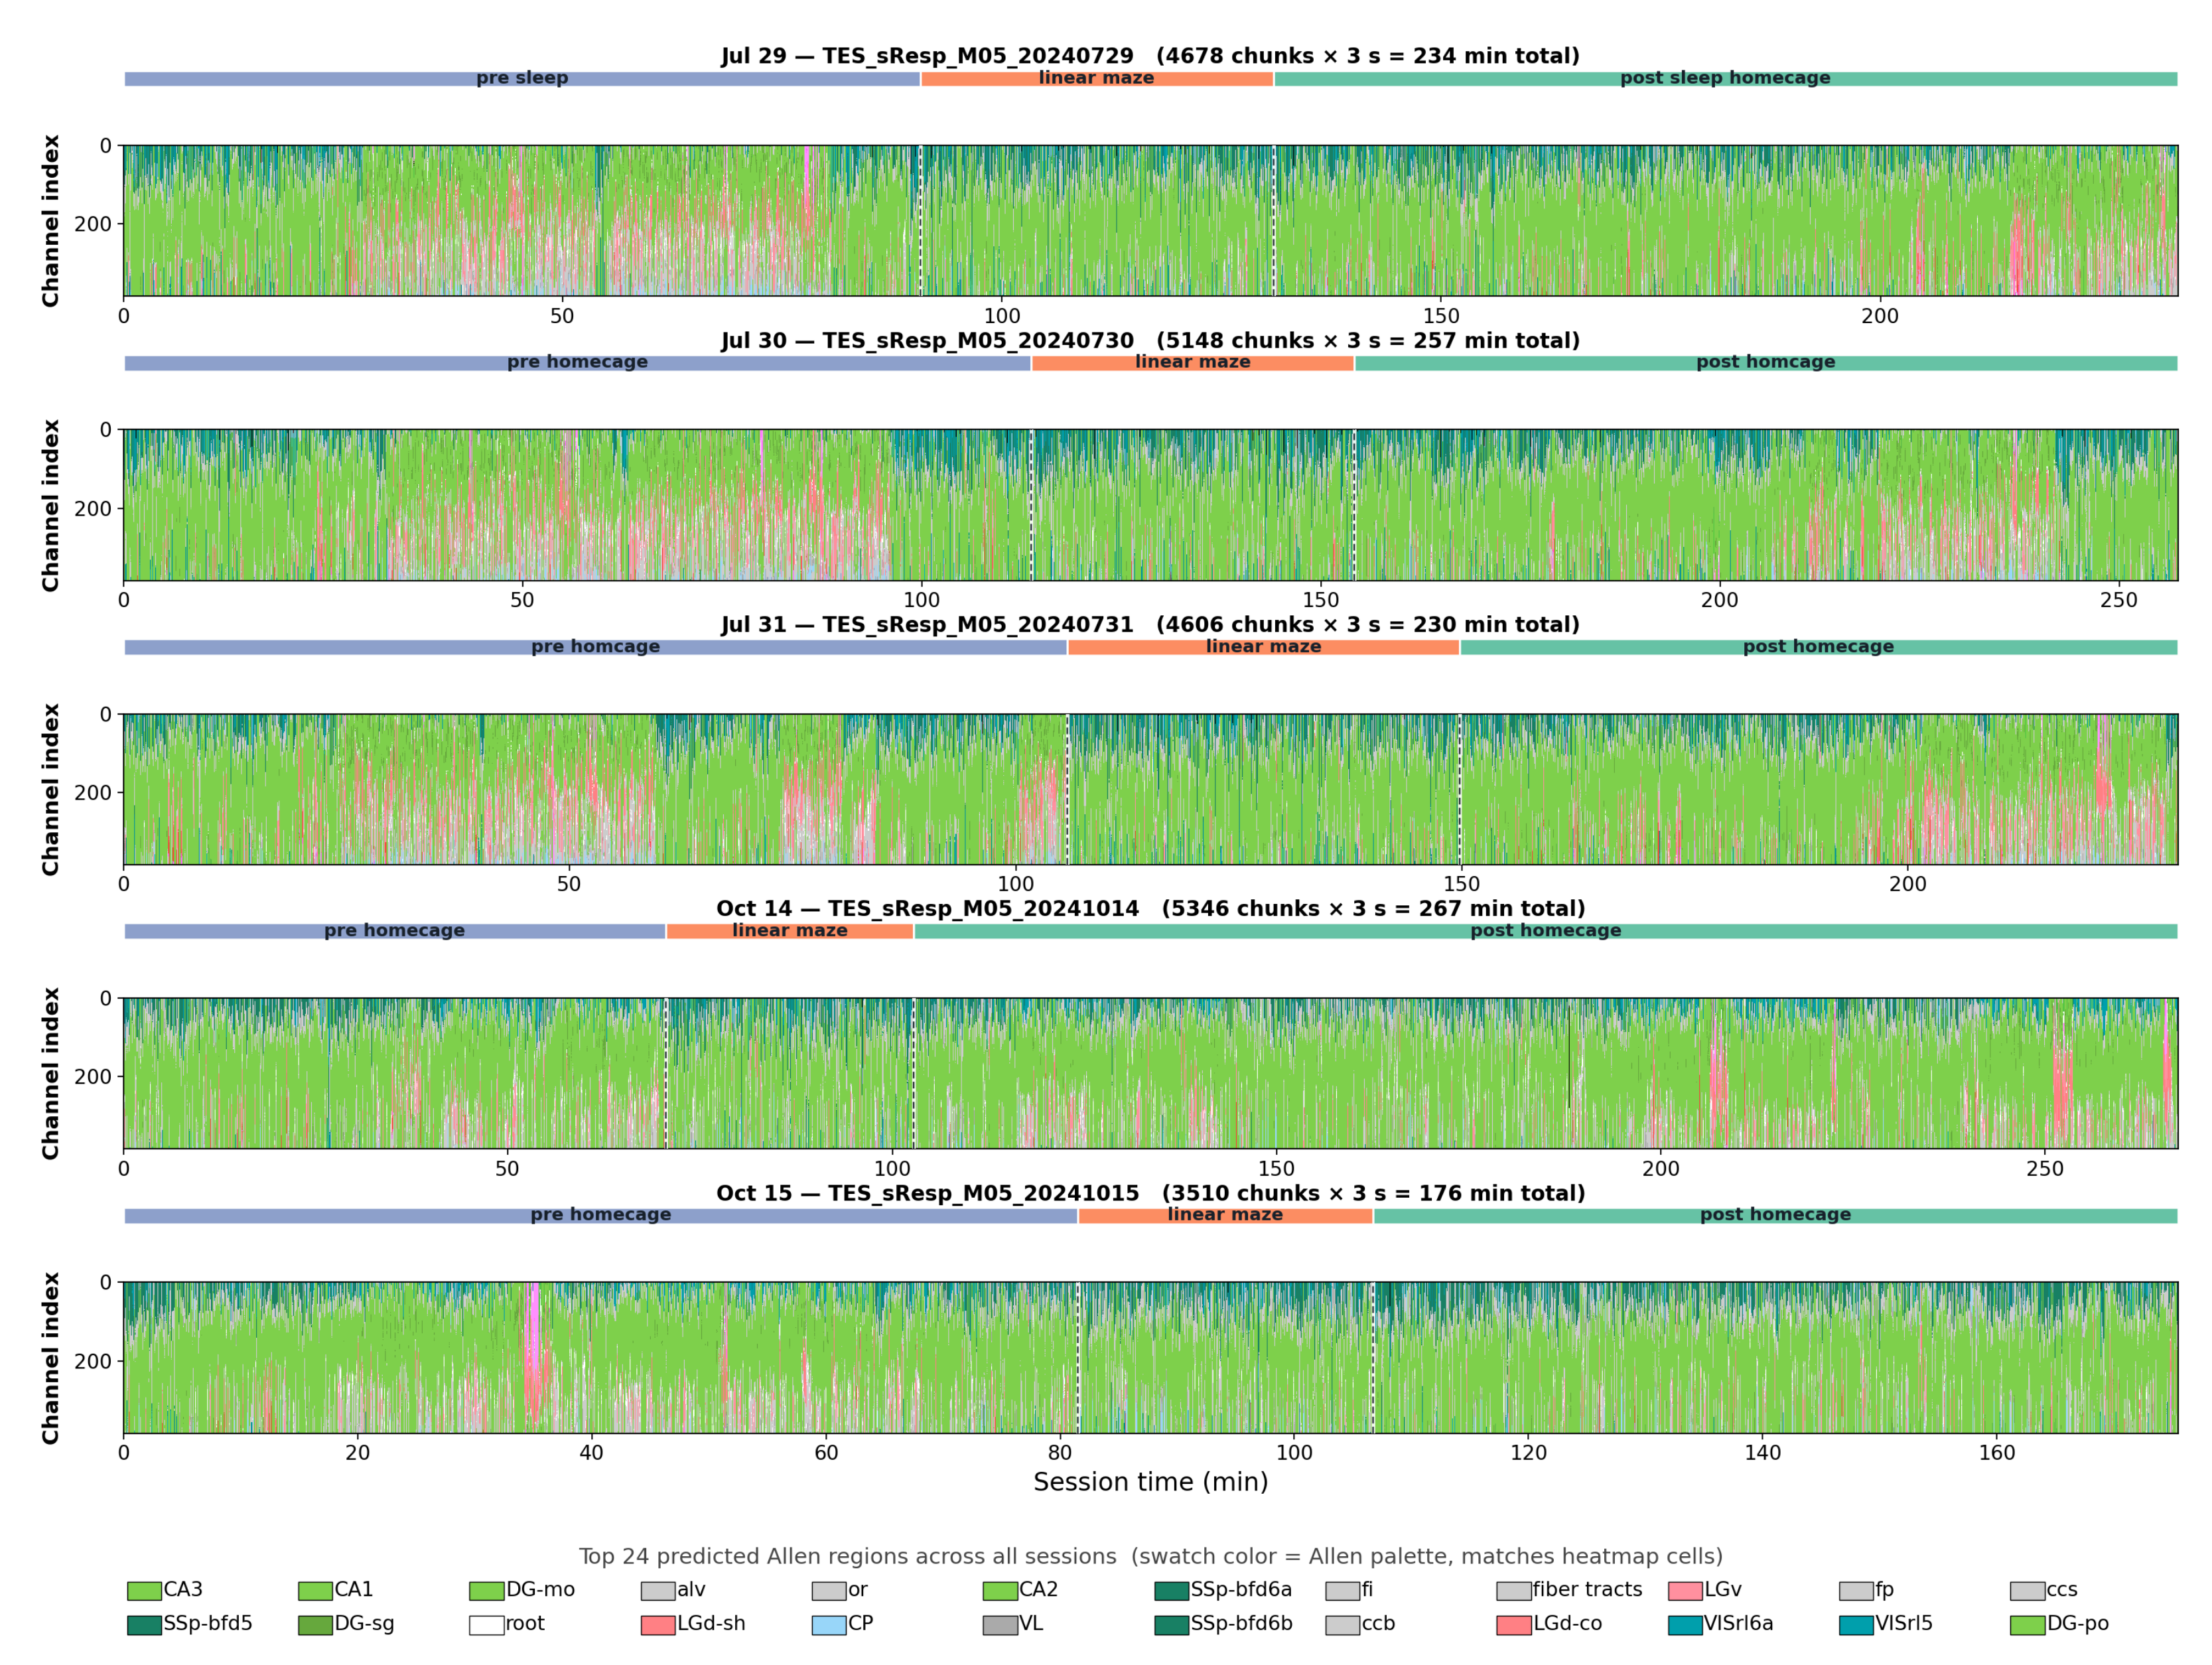
\includegraphics[width=\linewidth]{figures/supp_fig17_chronic_np2.png}
  \raggedright
  \vspace{-1.5ex}
  \begin{itemize}
    \item Five sessions (July, October; 19.4~h) from one mouse on a probe type and lab never seen in training; IBL-trained model, nothing fit to this animal.
    \item Predicted layout (deep cortex shallow, dorsal hippocampus along the shank) holds across hours and days; no histology, so consistency, not accuracy.
    \item Maze vs.\ home cage decoded at \textbf{0.863~$\pm$~0.036} vs.\ 0.692 for an elapsed-time control.
  \end{itemize}
\end{block}

\begin{block}{Conclusions and Limitations}
  \begin{itemize}
    \item Acquisition geometry is a useful, histology-free training signal for LFP foundation models.
    \item \MD{} and even \CD{} approach the \CCF{} oracle with Transformer readouts.
    \item LFP features and insertion records are complementary.
    \item The coordinate readout still needs anatomical labels, and $\sim$0.7--1~mm error is not yet a replacement for histology.
  \end{itemize}
\end{block}

\begin{block}{Code and References}
  \begin{minipage}[c]{0.22\linewidth}
    \qrcode[height=4.6cm]{https://www.neuroinformaticslab.com/lfpformer}
  \end{minipage}\hfill
  \begin{minipage}[c]{0.75\linewidth}
    \normalsize\raggedright
    \textbf{Project:} neuroinformaticslab.com/lfpformer\\
    \textbf{Code:} github.com/neuroinfolab/LFPformer\\
    \textbf{Encoders:} huggingface.co/Shubhronyu
  \end{minipage}

  \vspace{0.8ex}
  \footnotesize
  He et al., Lfp2vec, NeurIPS 2025 $\cdot$ Baevski et al., wav2vec 2.0, NeurIPS 2020 $\cdot$ IBL, Brain-Wide Map, Nature 2025 $\cdot$ Siegle et al., Nature 2021 $\cdot$ Kabsch, Acta Cryst.\ 1976 $\cdot$ Wang et al., bioRxiv 2025.
  Supported by NIMH R00MH128772, NINDS R00NS140554 and R01NS113782, and an NYU Google Cloud Research Award (RD157).
\end{block}

\end{column}
\separatorcolumn
\end{columns}
\end{frame}
\end{document}
